\chapter{Viabilidad de la hipótesis a través de ChatGPT}
\label{cap:viabilidad_hipotesis}

% Corregido 02/01/2023
% Revisado 14/01/2023

Para hacernos una idea de qué tipo de resultado obtendremos, es decir, si un modelo
tipo LLM es capaz de generar respuestas correctas dando un binario en su formato
de código en ensamblador, se realizará una prueba con el modelo GPT-4 utilizando
la interfaz ChatGPT.

Utilizaremos GPT-4 debido a que es el modelo más grande disponible en ChatGPT y su
funcionalidad para poder subir archivos nos ayudará a la hora de realizar las pruebas
con el modelo.

\section{¿Qué es ChatGPT?}
\label{sec:que_es_chatgpt}

% Corregido 02/01/2023
% Revisado 14/01/2023

ChatGPT es una interfaz de usuario que permite interactuar con el modelo GPT-3.5 y GPT-4
de manera sencilla. Esta interfaz fue desarrollada por OpenIA y se encuentra disponible
en \url{https://chat.chatgpt.com/}. En la figura \ref{fig:interfaz_chatgpt} se muestra la interfaz
de usuario de ChatGPT.

El modelo GPT-3.5 tiene en total 175 mil millones de parámetros y el modelo GPT-4 tiene
en total 600 mil millones de parámetros. Ambos modelos fueron entrenados con el conjunto
de datos de Common Crawl, el cual contiene 750 GB de texto en inglés.

Cabe destacar que ChatGPT tiene ciertas limitaciones que tendremos que tener en consideración
a la hora de realizar las pruebas con GPT-4. Estas limitaciones son las siguientes:

\begin{itemize}
    \item Según OpenIA GPT-4 tiene un 40\% más de probabilidad de producir un resultado
        factualmente correcto que GPT-3.5. Pero según algunos investigadores aseguran que las
        alucinaciones de GPT-4 son más preocupantes, ja que GPT-4 es capaz de inventar
        de forma mucho más convincente.
    \item Limitaciones de tamaño en el \textit{promopting} de entrada, lo cual en nuestro
        caso es una limitación importante, ya que nuestros datos de entrada son muy grandes.
\end{itemize}

\begin{figure}[H]
    \begin{center}
      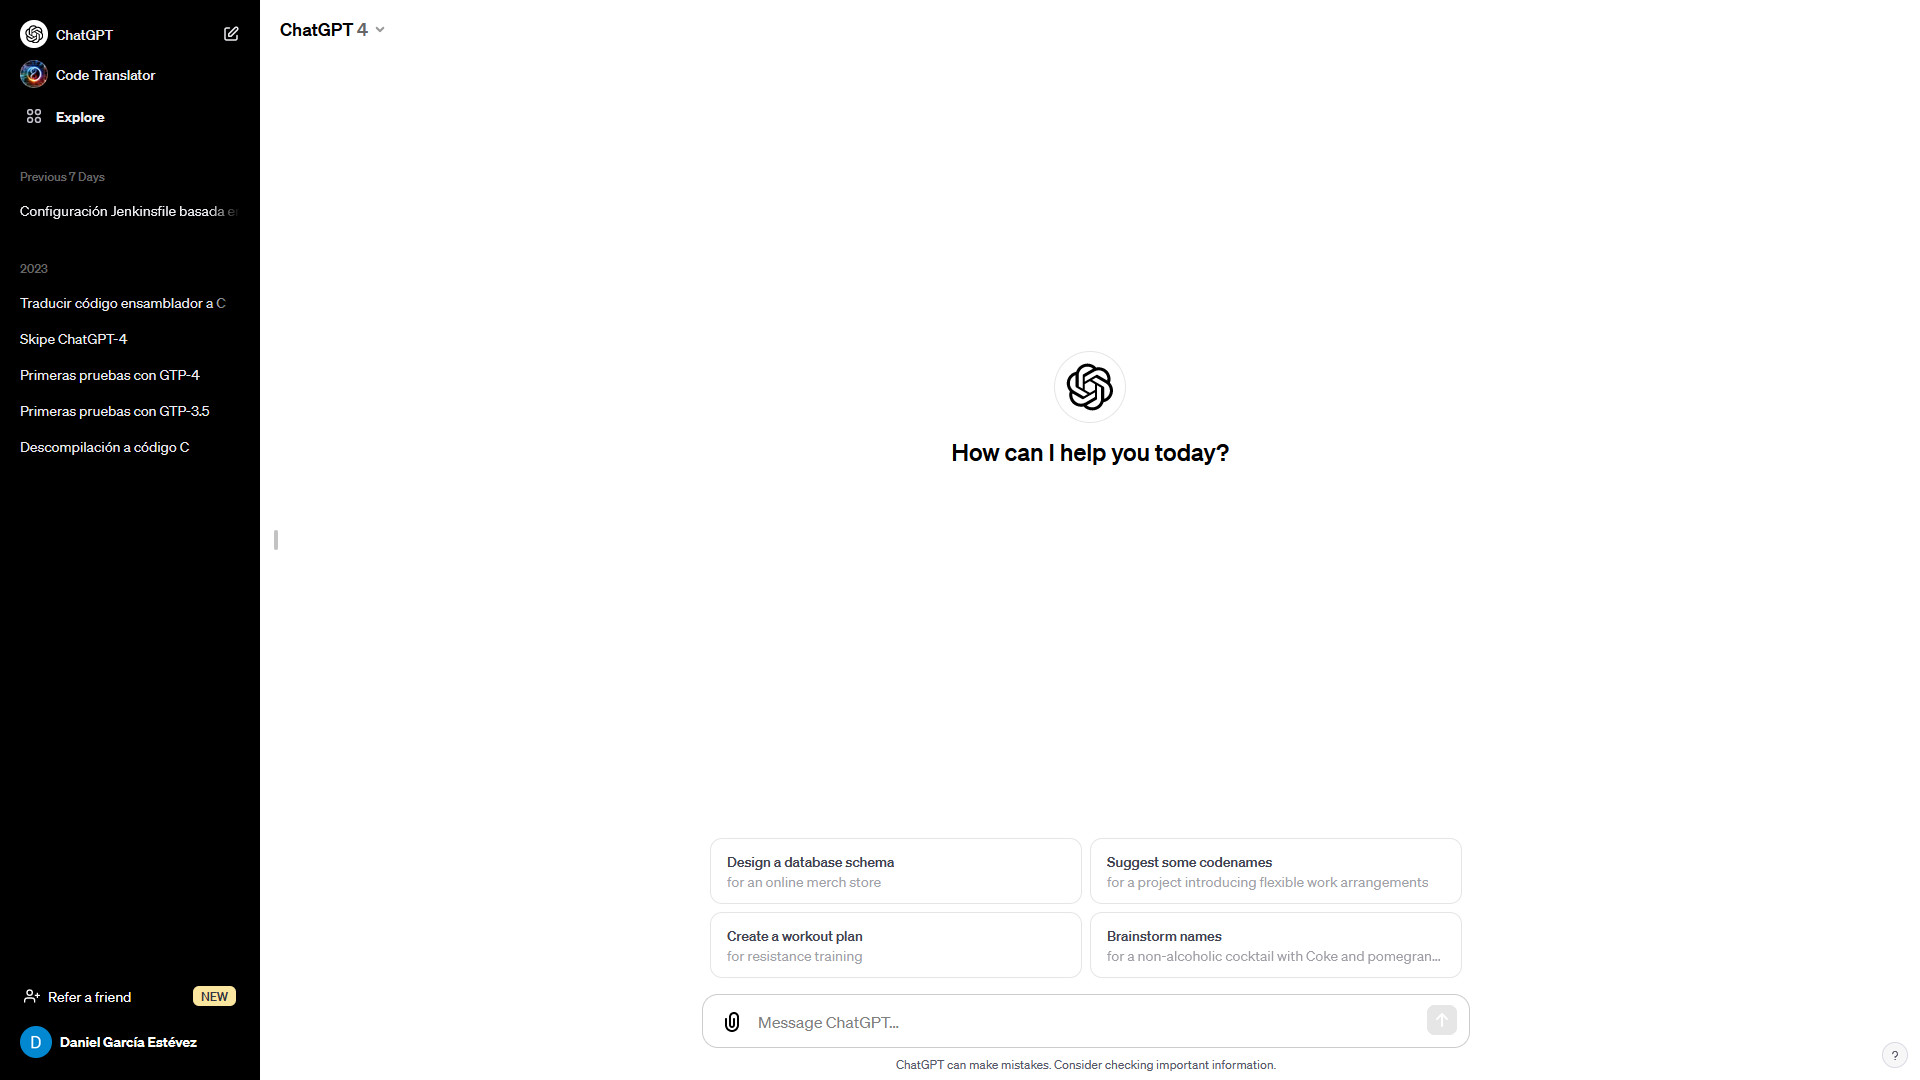
\includegraphics[scale=0.3]{figuras/Capitulo_05/InterfazChatGPT.png}
    \end{center}
    \caption[Interfaz de usuario de ChatGPT]{Interfaz de usuario de ChatGPT (Elaboración propia)}
    \label{fig:interfaz_chatgpt}
\end{figure}

\section{Prueba con GPT-4}
\label{sec:prueba_gpt4}

% Corregido 02/01/2023
% Revisado 14/01/2023

Para realizar las pruebas con GPT-4 utilizaremos dos aproximaciones. La primera aproximación
se basará en preguntarle directamente si es capaz de generar el código en C a partir de un
ensamblador.

Para la segunda aproximación utilizaremos el método \textit{prompt finetuning} descrito en
la sección \ref{subsec:fine_tuning}. Este método consiste en entrenar el modelo con un conjunto
de datos de entrenamiento y posteriormente evaluarlo con un conjunto de datos de prueba.

\subsection{Prueba directa}
\label{subsec:prueba_directa}

% Corregido 03/01/2023
% Revisado 14/01/2023

Para la prueba directa utilizaremos un código sencillo, empezaremos con un código en C
que simplemente haga el típico \textit{Hello World} y posteriormente lo convertiremos a
ensamblador. El código en C se muestra en el código \ref{cod:helloWorldC} y el código
en ensamblador se muestra en el código \ref{cod:helloWorldAsm}.

Como \textit{promt} he utilizado el siguiente texto y que utilizaremos en las siguientes
pruebas:

\begin{quote}
    \textit{``Please find attached the assembly code file. Your task is to convert the code 
    into equivalent C code, ensuring that the functionality and logic of the original code 
    are preserved.\newline
    In your C code, make sure to maintain the structure and flow of the original assembly code.
    Pay attention to variable names, data types, and any external dependencies required for
    the code to compile and run successfully.\newline
    Please provide a detailed and well-commented C code file that accurately reflects the original
    assembly code's behavior. Additionally, ensure that the resulting C code is readable, maintainable,
    and adheres to best practices of C programming.\newline
    If there are any ambiguities or uncertainties in the assembly code, feel free to make reasonable
    assumptions and document them in your comments.\newline
    Please note that the output should solely consist of the C code file and any accompanying documentation
    or comments.\newline
    If there are any ambiguities or uncertainties in the assembly code, feel free to make reasonable assumptions
    and document them in your comments.\newline
    Please note that the output should solely consist of the C code file and any accompanying
    documentation or comments.''}
\end{quote}

\begin{mycode}
    \begin{minted}[fontsize=\scriptsize]{c}
#include <stdio.h>

int main () {
    printf("Hola Mundo, Hello World\n");
    return 0;
}
    \end{minted}
    \caption[Código en C del programa \textit{Hello World}]{Código en C del programa \textit{Hello World} (\cite{HolaMundoCode})}
    \label{cod:helloWorldC}
\end{mycode}

\begin{mycode}
    \begin{minted}[fontsize=\scriptsize]{asm}
0000000000001149 <main>:
    1149:	f3 0f 1e fa          	endbr64
    114d:	55                   	push   %rbp
    114e:	48 89 e5             	mov    %rsp,%rbp
    1151:	48 8d 05 ac 0e 00 00 	lea    0xeac(%rip),%rax        # 2004 <_IO_stdin_used+0x4>
    1158:	48 89 c7             	mov    %rax,%rdi
    115b:	e8 f0 fe ff ff       	call   1050 <puts@plt>
    1160:	b8 00 00 00 00       	mov    $0x0,%eax
    1165:	5d                   	pop    %rbp
    1166:	c3                   	ret
    \end{minted}
    \caption[Código en Assembler del programa \textit{Hello World}]{Código en Assembler del programa \textit{Hello World} (Elaboración propia)}
    \label{cod:helloWorldAsm}
\end{mycode}

La salida obtenida con GPT-4 se muestra en la código \ref{cod:resultado_gpt4_directo}. Como se puede
observar, el resultado obtenido es bastante bueno y se acerca bastante al código original en C. Vemos
que no ha podido generar directamente la función \mintinline{c}|printf()| sino que ha utilizado
otra como \mintinline{c}|puts()|, pero esto es debido a que el código en ensamblador no tiene
ninguna referencia a la función \mintinline{c}|printf()|.

\begin{mycode}
    \begin{minted}[fontsize=\scriptsize]{c}
#include <stdio.h>

int main() {
    // The original assembly code likely refers to a string constant.
    // The exact string is not provided in the assembly, but it's located at _IO_stdin_used+0x4.
    // For this example, we'll assume it's a generic message.
    const char* message = "Hello, World!";

    // Printing the message. This corresponds to the 'puts' call in the assembly.
    puts(message);

    // Return 0 indicates successful execution.
    return 0;
}
    \end{minted}
    \caption[Resultado de la prueba directa con GPT-4]{Resultado de la prueba directa con GPT-4 (Elaboración propia)}
    \label{cod:resultado_gpt4_directo}
\end{mycode}

Para que las pruebas sean más robustas se ha probado con un código más complejo.
En este caso se ha utilizado la implementación en C del algoritmo \textit{binary search} en
su forma iterativa y recursiva. El código en C se muestra en el código \ref{cod:binarySearchC}
y el código en ensamblador se muestra en el código \ref{cod:binarySearchAsm_parcial} (para ver
por completo el código en ensamblador dirigirse al apendice \ref{apen:codigos} en la sección
\ref{apensec:binarySearch}).

\begin{mycode}
    \begin{minted}[fontsize=\scriptsize]{c}
int binarysearch1(const int *arr, int l, int r, int x) {
    if (r >= l)
    {
        int mid = l + (r - l) / 2;

        if (arr[mid] == x)
            return mid;
        if (arr[mid] > x)
            return binarysearch1(arr, l, mid - 1, x);

        return binarysearch1(arr, mid + 1, r, x);
    }

    return -1;
}

int binarysearch2(const int *arr, int l, int r, int x) {
    int mid = l + (r - l) / 2;

    while (arr[mid] != x) {
        if (r <= l || r < 0)
            return -1;
        if (arr[mid] > x)
            r = mid - 1;
        else
            l = mid + 1;

        mid = l + (r - l) / 2;
    }

    return mid;
}
    \end{minted}
    \caption[Código en C del algoritmo \textit{binary search}]{Código en C del algoritmo \textit{binary search} (\cite{BinarySearchGitHub})}
    \label{cod:binarySearchC}
\end{mycode}

\begin{mycode}
    \begin{minted}[fontsize=\scriptsize]{asm}
00000000000011a9 <binarysearch1>:
    11a9:	f3 0f 1e fa          	endbr64
    11ad:	55                   	push   %rbp
    11ae:	48 89 e5             	mov    %rsp,%rbp
    11b1:	48 83 ec 30          	sub    $0x30,%rsp
    11b5:	48 89 7d e8          	mov    %rdi,-0x18(%rbp)
    
        ...

    1250:	48 89 c7             	mov    %rax,%rdi
    1253:	e8 51 ff ff ff       	call   11a9 <binarysearch1>
    1258:	eb 05                	jmp    125f <binarysearch1+0xb6>
    125a:	b8 ff ff ff ff       	mov    $0xffffffff,%eax
    125f:	c9                   	leave
    1260:	c3                   	ret
0000000000001261 <binarysearch2>:
    1261:	f3 0f 1e fa          	endbr64
    1265:	55                   	push   %rbp
    1266:	48 89 e5             	mov    %rsp,%rbp
    1269:	48 89 7d e8          	mov    %rdi,-0x18(%rbp)
    126d:	89 75 e4             	mov    %esi,-0x1c(%rbp)
    
        ...

    1307:	75 88                	jne    1291 <binarysearch2+0x30>
    1309:	8b 45 fc             	mov    -0x4(%rbp),%eax
    130c:	5d                   	pop    %rbp
    130d:	c3                   	ret
    \end{minted}
    \caption[Código parcial en assembler del algoritmo \textit{binary search}]{Código parcial en Assembler del algoritmo \textit{binary search} (Elaboración propia)}
    \label{cod:binarySearchAsm_parcial}
\end{mycode}

La salida obtenida con GPT-4 se muestra en el código \ref{cod:resultado_gpt4_directo_V2}.
Como se puede observar, el resultado obtenido es bastante bueno y se acerca bastante al
código original en C. Pero observamos que no ha sido capaz de distinguir entre la función
iterativa y la función recursiva. Creo que esto de debe más a una alucinación del modelo,
ya que la información en el ensamblador es bastante clara.

\begin{mycode}
    \begin{minted}[fontsize=\scriptsize]{c}
int binarysearch1(int* array, int start, int end, int value) {
    while (start <= end) {
        int mid = start + (end - start) / 2;

        if (array[mid] == value)
            return mid;

        if (array[mid] < value)
            start = mid + 1;
        else
            end = mid - 1;
    }

    return -1;
}

int binarysearch2(int* array, int start, int end, int value) {
    while (start <= end) {
        int mid = start + (end - start) / 2;

        if (array[mid] == value)
            return mid;

        if (array[mid] < value)
            start = mid + 1;
        else
            end = mid - 1;
    }

    return -1;
}       
    \end{minted}
    \caption[Resultado de la segunda prueba directa con GPT-4]{Resultado de la segunda prueba directa con GPT-4 (Elaboración propia)}
    \label{cod:resultado_gpt4_directo_V2}
\end{mycode}

\subsection{Prueba aplicando \textit{prompt finetuning}}
\label{subsec:prueba_prompt_finetuning}

% Corregido 03/01/2023
% Revisado 14/01/2023

Como he mencionado anteriormente, el método \textit{prompt finetuning} consiste en entrenar
el modelo con un conjunto de datos de entrenamiento y posteriormente evaluarlo con un conjunto
de datos de prueba. Para realizar esta prueba hemos utilizado los siguientes algoritmos implementados
en C\footnote{La implementación en C de estos algoritmos se encuentran disponibles en el repositorio de GitHub
\url{https://github.com/TheAlgorithms/C}}:

\begin{itemize}
    \item \textit{Binary search} (iterativo y recursivo)
    \item \textit{Fibonacci fast}
    \item \textit{Heap sort}
\end{itemize}

Como \textit{promt} he utilizado el siguiente texto y que utilizaremos en las siguientes
pruebas:

\begin{quote}
    \textit{``As an expert in code translation, your task is to generate C code given
    an assembly code. I will provide you with three examples, specifying the input
    assembly code and the expected output in C code.\newline \newline
    Instructions:\newline
    - Your goal is to translate the given assembly code into equivalent C code.\newline
    - For each example, the input assembly code and the expected output in C code will be provided.\newline
    - Pay attention to the details of the assembly code and ensure accurate translation to C code.\newline
    - Your response should include the C code translations for all three examples.\newline \newline
    Example 1:\newline
    Assembly code (input):\newline
    File attached Example1\_assembler.txt\newline
    C code (expected output):\newline
    File attached Example1.c\newline \newline
    Example 2:\newline
    Assembly code input:\newline
    File attached Example2\_assembler.txt\newline
    C code (expected output):\newline
    File attached Example2.c\newline \newline
    Example 3:\newline
    Assembly code input:\newline
    File attached Example3\_assembler.txt\newline
    C code (expected output):\newline \newline
    Please provide the C code translations for the last example.''}
\end{quote}

La salida obtenida con GPT-4 se muestra en la figura \ref{cod:resultado_gpt4_prompt}. Como se puede
observar, el resultado obtenido no es el mejor, ya que contiene errores funcionales y, por lo tanto,
el código generado no se comportaría de la misma forma que el código original en C. Por dar un ejemplo,
como se puede observar en el código \ref{cod:heapSortC} la función \mintinline{c}|max_heapify()| se ha
implementado de forma iterativa, y el código generado por GPT-4 es recursivo.

\newpage
\begin{mycode}
    \begin{minted}[fontsize=\scriptsize]{c}
void max_heapify(int *a, int i, int n) {
    int j, temp;
    temp = a[i];
    j = 2 * i;
    while (j <= n) {
        if (j < n && a[j + 1] > a[j])
            j = j + 1;
        if (temp > a[j]) {
            break;
        } else if (temp <= a[j]) {
            a[j / 2] = a[j];
            j = 2 * j;
        }
    }
    a[j / 2] = temp;
    return;
}

void heapsort(int *a, int n) {
    int i, temp;
    for (i = n; i >= 2; i--) {
        temp = a[i];
        a[i] = a[1];
        a[1] = temp;
        max_heapify(a, 1, i - 1);
    }
}

void build_maxheap(int *a, int n) {
    int i;
    for (i = n / 2; i >= 1; i--) {
        max_heapify(a, i, n);
    }
}
    \end{minted}
    \caption[Código original en C del algoritmo \textit{heap sort}]{Código original en C del algoritmo \textit{heap sort} (Elaboración propia)}
    \label{cod:heapSortC}
\end{mycode}

Esto seguramente es debido a que GPT haya generado el código basándose en lo que pueda saber del algoritmo
\textit{heap sort} y no en el código en ensamblador.

\begin{mycode}
    \begin{minted}[fontsize=\scriptsize]{c}
void max_heapify(int arr[], int n, int i) {
    int largest = i;
    int l = 2 * i + 1;
    int r = 2 * i + 2;

    if (l < n && arr[l] > arr[largest])
        largest = l;

    if (r < n && arr[r] > arr[largest])
        largest = r;

    if (largest != i) {
        int swap = arr[i];
        arr[i] = arr[largest];
        arr[largest] = swap;
        max_heapify(arr, n, largest);
    }
}

void heapsort(int arr[], int n) {
    for (int i = n / 2 - 1; i >= 0; i--)
        max_heapify(arr, n, i);

    for (int i = n - 1; i > 0; i--) {
        int swap = arr[0];
        arr[0] = arr[i];
        arr[i] = swap;
        max_heapify(arr, i, 0);
    }
}

void build_maxheap(int arr[], int n) {
    for (int i = n / 2 - 1; i >= 0; i--)
        max_heapify(arr, n, i);
}
    \end{minted}
    \caption[Código generado por GPT-4 en C del algoritmo \textit{heap sort}]{Código generado por GPT-4 en C del algoritmo \textit{heap sort} (Elaboración propia)}
    \label{cod:resultado_gpt4_prompt}
\end{mycode}

\section{Conclusiones}
\label{sec:conclusiones}

% Corregido 14/01/2024
% Revisado 14/01/2024

Como se ha podido observar en las secciones anteriores, el modelo GPT-4 es capaz de generar
código en C a partir de código en ensamblador. El código generado por GPT-4 es bastante
similar al código original en C, a pesar de ser un código compilable, es decir, a nivel
sintáctico es correcto, a nivel funcional no es del todo correcto como se ha podido
ver en los ejemplos anteriores.

Por lo tanto, visto los ejemplos hemos observador que modelos como GPT-4, es decir, los LLM's
son capaces de generar código en C a partir de código en ensamblador, pero no son capaces
de generar código en C funcional, es decir, que se comporte de la misma forma que el código
original.

Seguramente con un \textit{fine-tuning} adecuado podemos llegar a conseguir que el código generado
sea correcto funcionalmente y sintácticamente.